\documentclass[11pt,a4paper]{article}

% ============ Packages ============
\usepackage[utf8]{inputenc}
\usepackage[T1]{fontenc}
\usepackage{amsmath,amssymb,amsthm}
\usepackage{mathtools}
\usepackage{graphicx}
\usepackage{booktabs}
\usepackage{tabularx}
\usepackage{hyperref}
\usepackage{cleveref}
\usepackage{listings}
\usepackage{xcolor}
\usepackage{geometry}
\usepackage{enumitem}
\usepackage{caption}
\usepackage{subcaption}
\usepackage{tikz}
\usetikzlibrary{shapes,shapes.geometric,arrows,arrows.meta,positioning,calc,fit,backgrounds,shadows}

\definecolor{kraftpaper}{RGB}{232, 215, 182}
\geometry{margin=1in}
\pagecolor{kraftpaper}
\color{black}

% ============ Theorem Environments ============
\newtheorem{theorem}{Theorem}[section]
\newtheorem{lemma}[theorem]{Lemma}
\newtheorem{corollary}[theorem]{Corollary}
\newtheorem{proposition}[theorem]{Proposition}
\newtheorem{definition}[theorem]{Definition}
\newtheorem{invariant}{Invariant}[section]

% ============ Listings ============
\definecolor{rustKeyword}{RGB}{204, 120, 50}
\definecolor{rustType}{RGB}{86, 156, 214}
\definecolor{rustComment}{RGB}{106, 153, 85}
\definecolor{rustString}{RGB}{206, 145, 120}
\definecolor{rustMacro}{RGB}{220, 220, 170}

\lstdefinelanguage{Rust}{
    keywords={fn, let, mut, pub, struct, enum, impl, self, Self, match, if, else, while, for, loop, return, break, continue, use, mod, crate, super, type, where, trait, as, const, static, ref, move, async, await, dyn, unsafe, extern},
    keywordstyle=\bfseries\color{rustKeyword},
    morekeywords=[2]{u8, u16, u32, u64, u128, i8, i16, i32, i64, i128, bool, String, Vec, HashMap, Option, Result, PublicKey, OutPoint, Signature},
    keywordstyle=[2]\color{rustType},
    morekeywords=[3]{ensure, derive},
    keywordstyle=[3]\color{rustMacro},
    sensitive=true,
    morecomment=[l]{//},
    morecomment=[s]{/*}{*/},
    commentstyle=\itshape\color{rustComment},
    morestring=[b]",
    stringstyle=\color{rustString},
}

\lstset{
    language=Rust,
    basicstyle=\footnotesize\ttfamily,
    keywordstyle=\bfseries\color{rustKeyword},
    commentstyle=\itshape\color{rustComment},
    stringstyle=\color{rustString},
    showstringspaces=false,
    breaklines=true,
    breakatwhitespace=true,
    frame=single,
    framerule=0.5pt,
    rulecolor=\color{gray!50},
    numbers=left,
    numberstyle=\tiny\color{gray},
    numbersep=5pt,
    stepnumber=1,
    tabsize=4,
    captionpos=b,
    aboveskip=8pt,
    belowskip=4pt,
    xleftmargin=12pt,
    framexleftmargin=10pt,
    columns=flexible,
    keepspaces=true,
}

% ============ Custom Commands ============
\newcommand{\bigO}{\mathcal{O}}
\newcommand{\calU}{\mathcal{U}}
\newcommand{\calS}{\mathcal{S}}
\newcommand{\code}[1]{\texttt{#1}}
\newcommand{\rfc}[1]{\textsc{#1}}
\newcommand{\RefOp}{\operatorname{Ref}}
\newcommand{\Fee}{\mathrm{Fee}}
\newcommand{\Hash}{\mathrm{H}}

% ============ Document Info ============
\title{Elone Prism: Merkleized Channels as Proof-First State Machines\\
\large Deterministic Settlement and Partition Conservation for Native Off-Chain State}
\author{
    Arthur Zhang\thanks{Corresponding author: Arthur Zhang (arthur@tondi.org)} \\
    \textit{Tondi Foundation}
}
\date{March, 2026}

\begin{document}
\maketitle

% ============ Abstract ============
\begin{abstract}
Existing off-chain channel systems often conflate three logically distinct concerns: the representation of channel state, the source of transaction fees, and the authorization boundary for unilateral settlement. The current Elone design already commits channel state through \code{balances\_root} and \code{ptlcs\_root}, but still relies on plaintext witnesses, local plaintext authority, and a \code{max\_fee} field embedded in the channel signing domain. This paper proposes a coherent refinement that completes the Merkleization of state and simultaneously eliminates channel-paid fees.

\textbf{Problem Statement:} Partial Merkleization is structurally unstable. If roots exist but validators still require plaintext state, the system inherits both the complexity of commitment-based state and the privacy leakage of plaintext-first execution. Likewise, removing \code{max\_fee} without introducing a stronger conservation rule would weaken the fee boundary rather than simplify it.

\textbf{Technical Contributions:} We make seven contributions. First, we define a \textbf{dual-subtree state commitment model} with separate balance and PTLC subtrees plus an optional aggregate root, together with a canonical \code{state\_header\_commitment}. Second, we introduce a \textbf{sponsor-paid fee model} in which channel value never pays fees. Third, we formalize \textbf{partition conservation}: exact conservation of channel-owned value and fee extraction exclusively from sponsor-owned value. Fourth, we distinguish \textbf{deterministic unilateral settlement} from \textbf{explicitly authorized cooperative settlement}, thereby repairing the output-authorization boundary of settlement flows. Fifth, we propose a \textbf{proof-first witness and storage model} in which local authority is expressed through roots, proofs, signatures, and encrypted leaf bundles rather than long-lived plaintext state. Sixth, we define \textbf{transition-footprint semantics} and show why proof-first validation is locality-preserving rather than full-state-reconstructive. Seventh, we characterize the \textbf{state package} as the correct recovery object: richer than a bare root, leaner than a permanent plaintext dump.

\textbf{Formal Consequences:} We show that partition conservation implies zero channel-paid fees and that deterministic settlement descriptors yield a unique unilateral settlement output set, up to canonical serialization. Under an explicit simple-proof model, we also show that proof-first verification is naturally local in the touched state footprint and that a bare state root is insufficient for unilateral recovery. These results replace fee-cap reasoning with a stronger invariant over value partitions and replace plaintext-authoritative recovery with a sharper notion of recoverable protocol meaning.

\textbf{Paper Type:} This draft should be read as a March 2026 protocol-design paper derived from the new Elone Merkle design memorandum. It is not a claim that the full design is already implemented, nor does it yet claim systems-level empirical closure. Rather, it provides a formalized architectural specification and migration discipline for upgrading Elone from a plaintext-assisted channel protocol to a proof-first, merkleized channel architecture.

\textbf{Keywords:} Payment Channels, Merkleized Channels, Partition Conservation, Proof-First Witnesses, Deterministic Settlement, Elone Protocol
\end{abstract}

\newpage
\tableofcontents
\newpage

% ============ Section 1 ============
\section{Introduction and Motivation}

Payment channel protocols require three properties simultaneously: low-latency off-chain state progression, enforceable unilateral settlement, and clear responsibility for transaction fees. In practice, these properties are frequently entangled. State is represented in one form for hashing and another for validation; fee budgets are embedded in signatures even when the intended policy is ``the channel itself should never pay fees''; and settlement outputs are often only partially authorized.

The new Elone Merkle design note of March 12, 2026 exposes this entanglement with unusual clarity. The current Elone codebase is not a system with ``no Merkle support.'' Rather, it is a system in which Merkle commitments already exist, but the protocol still behaves operationally as though plaintext channel state remains the authoritative witness. The result is a half-completed architecture: the system pays the conceptual cost of commitment-based state without fully obtaining its privacy, modularity, or proof-locality benefits.

This paper argues that the correct response is not a narrow local fix. Merkleization, sponsor-paid fees, and settlement authorization must be redesigned together. If only \code{max\_fee} is removed, the fee boundary becomes weaker. If only state storage is Merkleized but consensus still consumes plaintext witnesses, the protocol becomes more complex without becoming cleaner. If settlement outputs remain weakly authorized, sponsor-funded fees simply move the ambiguity to another layer.

Our central thesis is therefore:

\begin{quote}
\textit{A proof-first channel architecture requires simultaneous separation of state commitments, value conservation, and fee sponsorship.}
\end{quote}

This separation yields a more precise protocol language. Channel-owned value and sponsor-owned value become distinct partitions. Large, mutable collections move into Merkle subtrees. Hot metadata stays outside the tree. Unilateral settlement becomes descriptor-driven and deterministic. Cooperative settlement becomes explicitly committed. And the local authority model shifts from ``latest plaintext snapshot'' to ``latest signed roots plus proofs and encrypted leaf material.''

\subsection{Research Question}

The research question of this paper is not whether Merkle commitments can be applied to channel state in principle. That question has already been answered by the existence of the current dual-root Elone state format. The real question is sharper:

\begin{quote}
\textit{What protocol structure is required so that Merkleized state, sponsor-paid fees, and settlement authorization compose into a coherent channel system?}
\end{quote}

\subsection{Scope}

This paper focuses on the Elone protocol family. It does not attempt a general treatment of all payment channel systems. Nor does it claim that the entire design is already implemented in production code. The intended contribution is a research-level protocol refinement and migration target for Elone itself.

Accordingly, the present draft should be judged primarily as a protocol-design paper rather than as a finished systems paper. Where we introduce formal objects and propositions, the goal is to make the design auditable and extensible; where we do not yet provide empirical measurements, we say so explicitly and turn those gaps into a benchmark agenda rather than smuggling them in as implied evidence.

\subsection{Why This Requires a Dedicated Elone Paper}

This Merkle refinement is not a minor appendix to the earlier Elone state-machine paper. It changes the meaning of three protocol objects:
\begin{enumerate}
    \item \textbf{state}: from plaintext snapshots to commitment-authoritative state headers and proofs;
    \item \textbf{fee responsibility}: from bounded channel expenditure to strict channel-value conservation;
    \item \textbf{settlement authorization}: from builder-shaped output construction to descriptor-driven or root-bound authorization.
\end{enumerate}

For that reason, this document is best read as a dedicated Elone paper in its own right. The earlier Elone paper explains why native channel semantics belong at the consensus layer. \textbf{Elone Prism} explains how the next-generation state, witness, fee, and settlement objects should be structured once Merkle commitments become first-class protocol artifacts.

% ============ Section 2 ============
\section{Problem Statement and Current Snapshot}

\subsection{The Half-Merkle Problem}

The current Elone state object already contains two cryptographic commitments:
\begin{itemize}
    \item \code{balances\_root}
    \item \code{ptlcs\_root}
\end{itemize}

However, UPDATE and SETTLE validation still conceptually rely on plaintext state disclosure: validators reconstruct roots from explicit state payloads carried in the witness. This means the protocol still behaves as a plaintext-first protocol at validation time.

We call this the \textbf{half-Merkle problem}. A half-Merkle system simultaneously inherits:
\begin{enumerate}
    \item the protocol complexity of commitment-bearing state;
    \item the storage and privacy costs of plaintext authority;
    \item the ambiguity of deciding which layer truly owns the authoritative state.
\end{enumerate}

\subsection{The Fee-Boundary Problem}

The legacy Elone signing domain includes a fee cap. This structure implicitly encodes the proposition:
\[
\text{channel may pay up to some maximum fee.}
\]

But the target policy expressed in the new design note is categorically different:
\[
\text{channel pays no fee at all.}
\]

These are not equivalent formulations. A bounded channel-paid fee and a zero channel-paid fee induce different threat models. The former treats fee leakage as tolerable within limits; the latter treats fee leakage as a protocol violation.

\subsection{The Settlement-Authorization Problem}

Settlement is the point at which abstract state is turned back into spendable value. If settlement outputs are not strongly authorized, sponsor-funded fees do not solve the core problem; they merely relocate ambiguity. In particular, unilateral settlement cannot rely on ad hoc builder freedom. It requires a deterministic or explicitly committed output boundary.

\subsection{Current-vs-Proposed Interpretation}

\begin{table}[htbp]
\centering
\caption{Current Snapshot vs.\ Proposed Architecture}
\label{tab:current_vs_proposed}
\small
\begin{tabularx}{\linewidth}{@{}l X X@{}}
\toprule
\textbf{Dimension} & \textbf{Current Snapshot} & \textbf{Proposed Direction} \\
\midrule
State commitment & Dual roots exist, but plaintext witness still dominates validation & Proof-first validation over committed state subtrees \\
Fee model & \code{max\_fee} remains in the channel signing domain & Channel never pays fees; sponsor partition pays all fees \\
Settlement authorization & Output boundary is not yet the central protocol object & Timed settle is deterministic; coop settle signs a canonical output root \\
Local persistence & Plaintext state still behaves as local authority & Roots, proofs, signatures, and encrypted leaf bundles become authoritative \\
Protocol status & Partially implemented architecture & Research-grade refinement and migration target \\
\bottomrule
\end{tabularx}
\end{table}

\subsection{Three Competing Truths in the Legacy Direction}

The legacy direction implicitly contains three rival truth objects:
\begin{enumerate}
    \item the on-chain roots;
    \item the plaintext witness presented to validation;
    \item the plaintext state snapshot retained by local software.
\end{enumerate}

This is architecturally unstable. A protocol with multiple operational truths makes disagreement hard to localize: a failure may come from commitment construction, witness interpretation, or local storage drift. The Elone Prism direction intentionally collapses these truths into a single commitment-first authority:
\begin{quote}
\textit{the signed state header, together with admissible proofs and recovery material, is authoritative; plaintext is only cached interpretation.}
\end{quote}

% ============ Section 3 ============
\section{Research Contributions and Design Principles}

\subsection{Main Contributions}

This paper makes the following contributions:
\begin{enumerate}
    \item \textbf{Dual-Subtree State Commitment Model}: We formalize Elone state as separate balance and PTLC Merkle subtrees, with an optional aggregate root used as a cache key or protocol handle rather than an independent source of truth.
    \item \textbf{Sponsor-Paid Fee Architecture}: We define a fee model in which channel value is never used to pay fees, and all fee expenditure is isolated in sponsor-owned wallet inputs and change outputs.
    \item \textbf{Partition-Conservation Rule}: We replace fee-cap reasoning with exact value conservation over the channel partition and non-negative fee extraction from the sponsor partition.
    \item \textbf{Settlement Authorization Split}: We distinguish deterministic unilateral settlement from explicitly authorized cooperative settlement and explain why these two paths should not be represented by the same authorization object.
    \item \textbf{Proof-First Local Authority}: We redesign local persistence around roots, proofs, signatures, and encrypted leaves, thereby turning plaintext state from an authority object into a short-lived cache.
    \item \textbf{Transition-Footprint Semantics}: We model channel transitions through explicit read/write footprints and explain why proof-first witnesses should be evaluated by touched-state locality rather than by full-state reconstruction.
    \item \textbf{Recoverability as a Protocol Property}: We characterize the state package as the appropriate recovery object for unilateral enforceability, intermediate between a bare root and a full plaintext dump.
    \item \textbf{Phased Migration Discipline}: We provide a migration order that prioritizes authorization repair and fee-boundary repair before witness minimization and storage refactoring.
\end{enumerate}

\subsection{Design Principles}

The contributions above are organized by four design principles:
\begin{itemize}
    \item \textbf{Principle 1: Merkleize only large, mutable, proof-relevant collections.} Small, hot metadata should remain outside the tree.
    \item \textbf{Principle 2: Value conservation is stronger than fee caps.} If channel-owned value is exactly conserved, a fee cap becomes unnecessary.
    \item \textbf{Principle 3: Unilateral settlement must be deterministic.} The builder should not be a hidden authorization oracle.
    \item \textbf{Principle 4: Local authority should be commitment-first.} Plaintext is an optimization, not the ground truth.
    \item \textbf{Principle 5: Merkleization should improve locality, not merely hide bytes.} The decisive gain is not compression alone, but restricting validation and debugging to the touched portion of state.
\end{itemize}

% ============ Section 3.5 ============
\section{System Model and Threat Assumptions}

\subsection{Actors}

We assume four actor classes:
\begin{itemize}
    \item \textbf{Channel participants}, who jointly authorize off-chain state transitions.
    \item \textbf{Sponsors}, who provide ordinary wallet inputs to fund publication costs. A sponsor may be the same human or wallet operator as a channel participant, but it remains a distinct value role.
    \item \textbf{Consensus validators}, who decide admissibility of commitments, proofs, and value conservation.
    \item \textbf{Recovery runtimes}, which preserve signatures, proofs, and encrypted leaf material sufficient for continued operation or unilateral settlement.
\end{itemize}

\subsection{Adversarial Goals}

The adversary may attempt to:
\begin{enumerate}
    \item make channel-owned value silently absorb publication fees;
    \item exploit settlement-builder freedom to redirect unilateral outputs;
    \item exploit stale plaintext authority after commitment updates;
    \item manufacture proof-shape or witness-shape denial-of-service pressure.
\end{enumerate}

\subsection{Protocol Invariants}

\begin{invariant}[Commitment Authority]
Accepted protocol state must be derivable from the state header commitment and admissible proofs. Plaintext alone is never sufficient protocol authority.
\end{invariant}

\begin{invariant}[Channel Value Integrity]
No admissible Elone transaction may reduce the net value of the channel partition.
\end{invariant}

\begin{invariant}[Settlement Boundary Integrity]
For unilateral settlement, a valid state package and a fixed descriptor must determine a unique channel-owned output set, up to canonical serialization.
\end{invariant}

% ============ Section 4 ============
\section{Formal Transition Semantics}

\subsection{Channel Configuration}

We model a live Elone Prism channel at logical state number $t$ as a configuration
\[
\Gamma_t = (F, H_t, \Delta, \mathcal{B}_t, \mathcal{P}_t),
\]
where:
\begin{itemize}
    \item $F$ is the static fund anchor and channel identity context;
    \item $H_t$ is the canonical state header commitment at version $t$;
    \item $\Delta$ is the settlement descriptor family fixed or versioned by the channel;
    \item $\mathcal{B}_t$ is the canonical set of balance leaves committed by \code{balances\_root};
    \item $\mathcal{P}_t$ is the canonical set of PTLC leaves committed by \code{ptlcs\_root}.
\end{itemize}

Consensus never needs the full sets $(\mathcal{B}_t, \mathcal{P}_t)$ as explicit witness material. Instead, it needs only the protocol-relevant slice of those sets for the transition under evaluation. This is the key semantic shift from plaintext-first validation to proof-first validation.

\subsection{Transition Footprint}

\begin{definition}[Transition Footprint]
Let $\tau: \Gamma_t \rightarrow \Gamma_{t+1}$ be an UPDATE, SETTLE, or SPLICE transition. Its \textbf{transition footprint} is the tuple
\[
\Phi(\tau) = (R_B, R_P, W_B, W_P, M, A),
\]
where $R_B$ and $R_P$ are the balance and PTLC leaves read by the transition, $W_B$ and $W_P$ are the corresponding written or consumed leaves, $M$ is the tree-external metadata consumed by validation, and $A$ is the operation-specific authorization material.
\end{definition}

This definition clarifies a frequently blurred issue. A channel transition does not semantically depend on ``the whole state''; it depends on a bounded footprint plus the committed context in which that footprint is interpreted. Merkleization is therefore not merely a compression trick. It is a way of making the transition footprint explicit.

\begin{definition}[Admissible Proof-First Transition]
A transition $\tau: \Gamma_t \rightarrow \Gamma_{t+1}$ is \textbf{admissible} iff:
\begin{enumerate}
    \item every leaf in $R_B \cup R_P$ is justified by membership, emptiness, or non-membership proofs against $H_t$;
    \item the payloads in $W_B \cup W_P$ are canonically encoded and deterministically induce the next subtree roots in $H_{t+1}$;
    \item the authorization object $A$ binds the operation to the relevant header commitment and settlement boundary;
    \item the induced transaction satisfies partition conservation.
\end{enumerate}
\end{definition}

\subsection{Locality of Verification}

Let $N_B = |\mathcal{B}_t|$ and $N_P = |\mathcal{P}_t|$ be the cardinalities of the balance and PTLC sets, and let $k_B = |R_B| + |W_B|$ and $k_P = |R_P| + |W_P|$ be the effective touched-leaf counts of a transition.

\begin{proposition}[Local Verification Under a Simple Proof Model]
Assume fixed-arity canonical Merkle trees, bounded tree-external metadata, and no requirement to reconstruct untouched leaves. Then verification work for an admissible proof-first transition is
\[
\mathcal{O}(k_B \log N_B + k_P \log N_P + 1),
\]
rather than $\mathcal{O}(N_B + N_P)$ full-state reconstruction.
\end{proposition}

\begin{proof}
The verifier checks proofs only for the leaves named in the transition footprint. Each balance or PTLC proof has logarithmic length in the size of its corresponding canonical tree. Untouched leaves do not appear in the witness and are not reserialized. Tree-external metadata is bounded in size by protocol design. Therefore total verification work is proportional to the number of touched leaves times logarithmic proof length, plus constant-sized metadata checks.
\end{proof}

The academic significance of this theorem is broader than asymptotics. Locality narrows the epistemic surface of failure. When a transition is invalid, the disagreement is localized to the named footprint, its proofs, or its authorization boundary. In a plaintext-first system, disagreement can hide inside a much larger reconstructed state snapshot.

% ============ Section 5 ============
\section{Merkleized State Commitment Model}

\subsection{Dual Subtrees and Optional Aggregate Root}

We do not recommend a single flat state tree. Balance entries and PTLC entries have different update locality, different verification patterns, and different high-frequency predicates. In particular, the predicate
\[
\texttt{ptlcs\_root} = \texttt{EMPTY\_PTLCS\_ROOT}
\]
is operationally significant and should remain cheap to evaluate.

The proposed structure is:
\[
\texttt{state\_root} = \Hash(\texttt{version} \parallel \texttt{balances\_root} \parallel \texttt{ptlcs\_root}).
\]

The roots \code{balances\_root} and \code{ptlcs\_root} remain the semantically meaningful commitments. The optional \code{state\_root} is a derived aggregate handle. It must never become a competing source of truth.

\begin{definition}[State Header Commitment]
The \textbf{state header commitment} is the canonical hash of the protocol-visible channel state header:
\begin{align*}
\Hash(&\texttt{chain\_id} \parallel \texttt{channel\_id} \parallel \texttt{fund\_outpoint} \parallel \texttt{participants\_root} \\
      &\parallel \texttt{state\_number} \parallel \texttt{balances\_root} \parallel \texttt{ptlcs\_root} \\
      &\parallel \texttt{state\_layout\_version} \parallel \texttt{settlement\_descriptor\_root}).
\end{align*}
\end{definition}

\subsection{Tree-Internal vs.\ Tree-External Data}

The design memorandum correctly distinguishes \emph{large, mutable collections} from \emph{small, hot metadata}. The former should be Merkleized; the latter should remain tree-external.

\begin{table}[htbp]
\centering
\caption{Recommended State Placement}
\label{tab:state_placement}
\small
\begin{tabularx}{\linewidth}{@{}l X X@{}}
\toprule
\textbf{Category} & \textbf{Examples} & \textbf{Recommended Placement} \\
\midrule
Mutable state sets & balance leaves, PTLC leaves, settlement leaf material & Merkle subtrees \\
Hot metadata & \code{channel\_id}, \code{state\_number}, \code{csv\_delay}, \code{participants\_root} & Tree-external fields \\
Protocol versioning & \code{state\_layout\_version}, descriptor root & Tree-external, but committed via the state header \\
Wallet execution detail & sponsor inputs, sponsor change, coin selection trace & Never inside the channel state tree \\
\bottomrule
\end{tabularx}
\end{table}

\subsection{State Carrier Reserve}

The value previously described operationally as \code{state\_utxo\_value} should not be treated as business logic or fee budget. Under the proposed model it is demoted to a technical reserve:
\[
\texttt{state\_carrier\_reserve} = \max(\texttt{MIN\_STATE\_UTXO\_VALUE}, \texttt{layout\_specific\_minimum}).
\]

Its role is purely to satisfy base-layer state-carrier requirements. It must:
\begin{enumerate}
    \item remain outside the signing semantics of off-chain balance evolution;
    \item never be interpreted as channel fee budget;
    \item be fully conserved or refunded according to transaction type.
\end{enumerate}

\subsection{Canonical Leaf Discipline}

Merkleization is not merely a storage compression technique; it is a semantics discipline. Let each balance leaf and PTLC leaf carry a canonical ordering key determined by protocol rules rather than by local insertion order. Then:
\begin{align*}
\texttt{balances\_root} &= \Hash(\texttt{sorted balance leaves}), \\
\texttt{ptlcs\_root} &= \Hash(\texttt{sorted PTLC leaves}).
\end{align*}

This canonicalization requirement has an important theoretical consequence: the protocol ceases to interpret Merkle roots as opaque hashes and instead interprets them as \emph{canonical summaries of a uniquely ordered state set}. Without canonical leaf order, two semantically identical local states could still diverge at the commitment layer.

\subsection{Proof Objects as First-Class Protocol Objects}

The proof-first model requires more than ``some Merkle proofs.'' We distinguish three first-class protocol objects:
\begin{enumerate}
    \item \textbf{StateAccessManifest}: the declaration of which subtrees and leaves are relevant to the transition;
    \item \textbf{MerkleProofBundle}: the membership, emptiness, or non-membership proofs that justify those declarations;
    \item \textbf{LeafPayloadBundle}: the canonical payload material whose hashes realize the claimed leaves.
\end{enumerate}

The academic insight here is that a proof-first channel protocol should treat \emph{proof shape} as part of protocol meaning, not merely as SDK serialization. Once state access becomes partial and structured, the witness itself becomes a constrained proof object rather than a bag of implementation detail.

\begin{figure}[htbp]
\centering
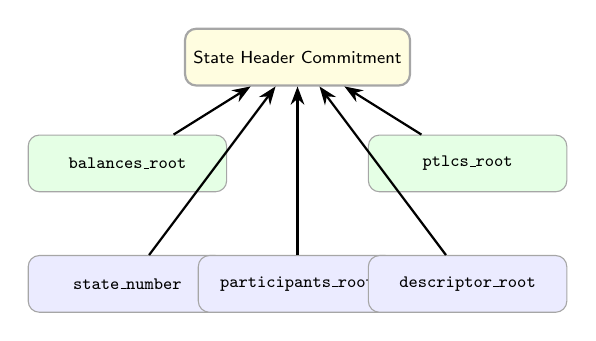
\begin{tikzpicture}[
    scale=0.9, transform shape,
    font=\sffamily\scriptsize,
    box/.style={rectangle, draw=gray!70, rounded corners, minimum width=2.8cm, minimum height=0.8cm, fill=white},
    root/.style={box, fill=yellow!12, thick},
    subtree/.style={box, fill=green!10},
    meta/.style={box, fill=blue!8},
    arrow/.style={->, >=Stealth, thick}
]
    \node[root] (state) at (0,3.2) {State Header Commitment};
    \node[subtree] (balances) at (-2.4,1.7) {\code{balances\_root}};
    \node[subtree] (ptlcs) at (2.4,1.7) {\code{ptlcs\_root}};
    \node[meta] (meta1) at (-2.4,0) {\code{state\_number}};
    \node[meta] (meta2) at (0,0) {\code{participants\_root}};
    \node[meta] (meta3) at (2.4,0) {\code{descriptor\_root}};

    \draw[arrow] (balances) -- (state);
    \draw[arrow] (ptlcs) -- (state);
    \draw[arrow] (meta1) -- (state);
    \draw[arrow] (meta2) -- (state);
    \draw[arrow] (meta3) -- (state);
\end{tikzpicture}
\caption{Proof-first Elone state: large mutable sets are Merkleized, while hot metadata remains tree-external but commitment-bound.}
\label{fig:state_header_commitment}
\end{figure}

% ============ Section 6 ============
\section{Sponsor-Paid Fees and Partition Conservation}

\subsection{Initialization vs.\ Post-Funding Transitions}

FUND is not semantically identical to UPDATE, SETTLE, or SPLICE. FUND creates the initial channel partition from ordinary wallet-owned value. By contrast, UPDATE, SETTLE, and SPLICE transform an already existing channel partition. This distinction matters because exact channel-partition conservation is a property of \emph{post-funding channel transitions}, not of the initial funding act itself.

We therefore distinguish:
\begin{itemize}
    \item \textbf{initialization}: FUND creates channel-owned outputs from setup-wallet value and pays fees in the ordinary wallet manner;
    \item \textbf{post-funding transitions}: UPDATE, SETTLE, and SPLICE preserve the already created channel partition while allowing sponsor-funded publication.
\end{itemize}

\subsection{Partitioned Value Semantics}

Every post-funding Elone transition is divided into two value partitions:
\begin{itemize}
    \item the \textbf{channel partition}, consisting of channel-owned inputs and channel-owned outputs;
    \item the \textbf{sponsor partition}, consisting of ordinary wallet inputs and ordinary sponsor change outputs.
\end{itemize}

This division is semantic rather than script-template-based. In particular, cooperative settlement may produce ordinary address outputs that nonetheless belong to the channel partition. Therefore, partition membership cannot be determined by superficial output shape. It must be determined by commitment membership or deterministic derivation.

\subsection{Partition Assignment Semantics}

\begin{definition}[Partition Map]
For each post-funding Elone transition $T$, the protocol defines a deterministic map
\[
\pi_T : E(T) \rightarrow \{C, S, R\},
\]
where $E(T)$ is the set of transaction-relevant elements, $C$ denotes channel-owned value, $S$ denotes sponsor-owned value, and $R$ denotes reference-only elements that affect validation but do not enter value conservation.
\end{definition}

The crucial role of $\pi_T$ is to prevent partition assignment from degenerating into output-shape heuristics. The map is part of protocol semantics, not wallet convention.

\begin{table}[htbp]
\centering
\caption{Deterministic Partition Assignment for Post-Funding Transitions}
\label{tab:partition_assignment}
\small
\begin{tabularx}{\linewidth}{@{}l X X X@{}}
\toprule
\textbf{Tx Type} & \textbf{Channel-Owned ($C$)} & \textbf{Sponsor-Owned ($S$)} & \textbf{Reference-Only ($R$)} \\
\midrule
UPDATE & consumed \code{ChannelState}; created next \code{ChannelState} & sponsor wallet inputs and sponsor change outputs & \code{ChannelFundRef} context input \\
Timed SETTLE & consumed \code{ChannelFund} and \code{ChannelState}; all outputs from descriptor derivation & optional sponsor wallet inputs and sponsor change outputs & none \\
Coop SETTLE & consumed \code{ChannelFund} and \code{ChannelState}; outputs committed by \code{settle\_outputs\_root} & optional sponsor wallet inputs and sponsor change outputs not covered by that root & none \\
SPLICE & all consumed and created channel-typed topology outputs designated by splice commitments & sponsor wallet inputs and sponsor change outputs & topology references with no spend value \\
\bottomrule
\end{tabularx}
\end{table}

FUND is exceptional. It creates the initial channel partition by moving setup-wallet value into \code{ChannelFund} and \code{ChannelState(0)} outputs. Fees are still wallet-funded, but exact conservation is not yet defined over a pre-existing channel partition because none exists before funding.

\begin{definition}[Partition Conservation]
Let $T$ be a post-funding Elone transition. Let $V_C^{in}(T)$ and $V_C^{out}(T)$ denote the total input and output value of the elements for which $\pi_T(e)=C$. Let $V_S^{in}(T)$ and $V_S^{out}(T)$ denote the corresponding totals for the elements for which $\pi_T(e)=S$. The transition satisfies \textbf{partition conservation} iff:
\[
V_C^{in}(T) = V_C^{out}(T)
\]
and
\[
V_S^{in}(T) \geq V_S^{out}(T).
\]
The fee is then defined as:
\[
\Fee(T) = V_S^{in}(T) - V_S^{out}(T).
\]
\end{definition}

\begin{proposition}[Channel Fee Isolation]
If partition conservation holds, then channel-owned value never pays transaction fees.
\end{proposition}

\begin{proof}
By definition, $V_C^{in}(T) = V_C^{out}(T)$. Therefore no value deficit is introduced within the channel partition of $T$. Since total fee is defined entirely by the sponsor deficit $V_S^{in}(T) - V_S^{out}(T)$, all fees must be paid by the sponsor partition. Hence channel-paid fee is identically zero.
\end{proof}

\begin{corollary}
Under partition conservation, a channel fee cap is not a primary safety invariant.
\end{corollary}

\subsection{Why Fee Caps Are Insufficient}

A fee cap bounds channel loss; it does not prohibit channel loss. The sponsor-paid model aims to forbid channel fee expenditure rather than merely constrain it. This is a categorical difference in protocol semantics. Consequently:
\begin{enumerate}
    \item deleting \code{max\_fee} without partition conservation is unsafe;
    \item keeping \code{max\_fee} after partition conservation is conceptually redundant.
\end{enumerate}

\subsection{Why Sponsorship Remains Central Even If the Title Changes}

This paper does not foreground sponsor-paid fees in its title because the deeper conceptual object is the merkleized channel itself. Nevertheless, sponsorship remains central to the protocol logic. Once channel-owned value is defined to be exactly conserved, some other partition must bear publication cost. The sponsor abstraction is therefore not cosmetic wallet terminology; it is the value-theoretic complement of channel conservation.

% ============ Section 7 ============
\section{Transaction Semantics Under the New Model}

\subsection{FUND}

FUND remains the least controversial path. It already uses wallet-owned inputs and can therefore continue to fund its own fees in the usual base-layer manner. The important change is architectural: FUND should fix the long-lived settlement descriptor and state layout anchors early, rather than leaving settlement boundary semantics implicit.

\subsection{Legacy vs.\ Elone Prism Semantics}

\begin{table}[htbp]
\centering
\caption{Legacy Direction vs.\ Elone Prism}
\label{tab:legacy_vs_prism}
\small
\begin{tabularx}{\linewidth}{@{}l X X@{}}
\toprule
\textbf{Aspect} & \textbf{Legacy Direction} & \textbf{Elone Prism Direction} \\
\midrule
State authority & Plaintext snapshots dominate operational truth & State headers and proofs dominate operational truth \\
Witness model & Plaintext-assisted & Access-scoped and proof-first \\
Fee semantics & Channel loss is capped & Channel loss is prohibited by conservation \\
Settlement semantics & Builder freedom remains substantial & Descriptor or output-root binds the boundary \\
Recovery object & Latest local state dump & State package with proofs and encrypted leaves \\
\bottomrule
\end{tabularx}
\end{table}

\subsection{UPDATE}

The proposed UPDATE consumes the previous state carrier and references the fund anchor:
\begin{itemize}
    \item channel inputs: \code{ChannelStateSpend} and \code{ChannelFundRef};
    \item sponsor inputs: ordinary wallet UTXOs, if fees must be paid;
    \item outputs: the new \code{ChannelState} plus sponsor change.
\end{itemize}

The state carrier reserve is preserved:
\[
\texttt{old\_state\_value} = \texttt{new\_state\_value}.
\]
The fee is paid exclusively by sponsor inputs.

\begin{lstlisting}[caption={Proof-First UPDATE Witness Sketch}, float=!htb]
pub struct UpdateWitnessVNext {
    pub state_header_commitment: [u8; 32],
    pub access_manifest: StateAccessManifest,
    pub proof_bundle: MerkleProofBundle,
    pub touched_leaf_payloads: Vec<Vec<u8>>,
    pub agg_signature: Signature,
}
\end{lstlisting}

\subsection{SETTLE}

SETTLE is the most security-sensitive path because it converts committed state into spendable outputs. We separate two modes:

\paragraph{Timed / unilateral settle.}
The unilateral path should not permit arbitrary builder freedom. Its outputs must be uniquely derivable from:
\begin{enumerate}
    \item the proved channel state;
    \item the participants commitment;
    \item the settlement descriptor.
\end{enumerate}

\begin{proposition}[Deterministic Timed Settle]
Given a valid state proof, a fixed settlement descriptor, and a canonical serialization rule, the unilateral settlement output set is unique.
\end{proposition}

\begin{proof}[Proof sketch]
The descriptor specifies the authorized settlement transformation. The proved leaves determine balances and any required PTLC emptiness predicates. Canonical serialization removes builder discretion. Therefore the resulting channel-owned output multiset is uniquely determined.
\end{proof}

\paragraph{Cooperative settle.}
The cooperative path may intentionally expose more flexibility for address rotation, output coalescing, or dust management. That flexibility must be bounded by an explicit channel-owned output commitment:
\[
\texttt{settle\_outputs\_root}.
\]
Sponsor change outputs must remain outside this commitment.

This split matches an important asymmetry already visible in the current Elone validator. Timed settle enforces commitment consistency against the on-chain state carrier, whereas cooperative settle can authorize a later mutually signed off-chain state without first publishing an intermediate UPDATE. Elone Prism does not erase that asymmetry; it makes it explicit and gives each path a distinct authorization object.

\subsection{Settlement Descriptor as a Protocol Object}

The settlement descriptor is the bridge between abstract state commitments and concrete value redistribution. A useful descriptor should specify:
\begin{enumerate}
    \item participant destination policy;
    \item unilateral derivation rules;
    \item cooperative canonicalization rules;
    \item versioning hooks for future settlement evolution.
\end{enumerate}

This yields a clean academic separation:
\begin{itemize}
    \item \textbf{Timed settle}: the descriptor acts as an algorithmic specification.
    \item \textbf{Coop settle}: the descriptor constrains a separately signed \code{settle\_outputs\_root}.
\end{itemize}

The descriptor is thus neither a mere wallet hint nor a generic scripting language. It is a narrow authorization object whose purpose is to eliminate hidden builder discretion.

\subsection{A Minimal Descriptor Calculus}

To make the descriptor auditable, we define a minimal descriptor grammar:
\[
\Delta = (\texttt{version}, \texttt{participants}, \rho_{\mathrm{pay}}, \rho_{\mathrm{ptlc}}, \rho_{\mathrm{asset}}, \rho_{\mathrm{coop}}),
\]
where:
\begin{itemize}
    \item \texttt{participants} fixes the participant set and destination identities available to the channel;
    \item $\rho_{\mathrm{pay}}$ maps proved balance leaves to canonical payout instructions;
    \item $\rho_{\mathrm{ptlc}}$ specifies the PTLC emptiness or resolution predicates required before timed settlement is admissible;
    \item $\rho_{\mathrm{asset}}$ specifies asset-aware routing and output grouping policy;
    \item $\rho_{\mathrm{coop}}$ specifies the canonicalization rule for cooperative output commitments.
\end{itemize}

The point of this calculus is not to create a general-purpose scripting language. It is to specify precisely which degrees of freedom are allowed to influence settlement and which are not.

\subsection{Descriptor Commitment and Upgrade Boundaries}

The descriptor root belongs in the state header commitment because it changes the meaning of settlement, not merely its serialization. Two consequences follow:
\begin{enumerate}
    \item if the descriptor root changes, the channel has changed one of its authorization objects, and the change must therefore be reflected in a new authorized state header;
    \item a state package remains recoverable across time only relative to the descriptor version committed by that package.
\end{enumerate}

This is why descriptor upgrades cannot be treated as wallet-local metadata edits. They are semantic upgrades to the settlement calculus itself.

\subsection{Timed-Settle Derivation}

The minimal deterministic derivation rule can be expressed as follows.

\begin{lstlisting}[caption={Timed-Settle Output Derivation Sketch}, float=!htb]
fn derive_timed_settle_outputs(
    package: &StatePackage,
    descriptor: &Descriptor
) -> Result<Vec<Output>, Error> {
    require(package.descriptor_root == descriptor.commitment());
    require(descriptor.ptlc_rule.admits(&package.ptlc_proofs)?);

    let mut outputs = vec![];
    for leaf in package.balance_leaves.iter().sorted_by_key(canonical_key) {
        outputs.push(descriptor.payout_rule.to_output(leaf)?);
    }

    descriptor.asset_policy.normalize(&mut outputs)?;
    descriptor.coop_policy.assert_not_required()?;
    canonical_serialize(outputs)
}
\end{lstlisting}

The important fact about this pseudocode is not its surface syntax. It is that no hidden builder discretion remains once the state package and descriptor are fixed. That property is exactly what unilateral settlement needs.

\subsection{SPLICE}

SPLICE preserves exact channel-owned value across channel topology transitions while permitting sponsor-funded fees. The semantic equation is:
\[
\sum \text{consumed channel-owned values} = \sum \text{created channel-owned values}.
\]

From an engineering perspective, SPLICE should not be the first path to receive maximal proof optimization. UPDATE and SETTLE should be stabilized first, because SPLICE magnifies every unresolved boundary in the system.

\begin{table}[htbp]
\centering
\caption{Transaction-Level Effect of the New Model}
\label{tab:tx_semantics}
\small
\begin{tabularx}{\linewidth}{@{}l X X@{}}
\toprule
\textbf{Tx Type} & \textbf{Channel Semantics} & \textbf{Sponsor Semantics} \\
\midrule
FUND & Creates \code{ChannelFund} and \code{ChannelState(0)} & Ordinary wallet funding path \\
UPDATE & State carrier reserve migrates 1:1 into the next state & Sponsor covers fee and receives sponsor change \\
SETTLE & All channel-owned value must appear in authorized channel settlement outputs & Optional sponsor covers fee only \\
SPLICE & Channel-owned value is exactly redistributed across topology outputs & Sponsor covers fee without altering net channel value \\
\bottomrule
\end{tabularx}
\end{table}

% ============ Section 8 ============
\section{Proof-First Witness and Local Persistence}

\subsection{From Plaintext Authority to Commitment Authority}

The local authority object should no longer be a pair of plaintext vectors:
\begin{itemize}
    \item \code{Vec<BalanceEntry>}
    \item \code{Vec<PtlcEntry>}
\end{itemize}

Instead, the authoritative local object becomes:
\begin{itemize}
    \item the latest state number;
    \item the latest signed state header commitment;
    \item proof inventory;
    \item signature inventory;
    \item encrypted leaf material sufficient for recovery.
\end{itemize}

\subsection{Recommended Storage Layers}

We adopt the following four-layer local storage model:
\begin{enumerate}
    \item \textbf{Channel tip metadata:} state number, roots, signatures, and descriptor version.
    \item \textbf{Merkle node cache:} optional node material indexed by hash.
    \item \textbf{Encrypted leaf bundle store:} serialized balance/PTLC/descriptor leaf payloads.
    \item \textbf{Secret vault:} adaptor material, revealed secrets, and local recovery-only secrets.
\end{enumerate}

The paper does not recommend an aggressively abstract graph database for Merkle nodes as the first implementation target. Correctness, recoverability, and predictable garbage collection are more important than maximal generality in version one.

\subsection{State Package as the New Recovery Unit}

To make commitment authority operational, we define a \textbf{state package} as the minimal recoverable object that permits a participant to continue operating or to settle:
\begin{enumerate}
    \item the state header commitment and version fields;
    \item the latest aggregated signatures needed for admissible next actions;
    \item the proofs required for those next actions;
    \item the encrypted leaf material required to reconstruct or interpret those proofs.
\end{enumerate}

This object is richer than a bare root and leaner than a permanent plaintext state dump. That is precisely why it is the correct recovery object: it preserves protocol meaning without reintroducing plaintext authority as a long-lived invariant.

\subsection{Privacy Interpretation}

The goal is not ``never persist plaintext in any circumstance.'' The realistic goal is stronger and more operational:
\begin{enumerate}
    \item plaintext should not be the default authority object;
    \item crash recovery should not require plaintext snapshots;
    \item any plaintext cache should be local, short-lived, and encrypted when persisted.
\end{enumerate}

\section{Recoverability as a Protocol Property}

\subsection{Bare Roots, Plaintext Dumps, and State Packages}

A bare root is compact, but semantically thin. A plaintext dump is semantically rich, but operationally heavy and privacy-hostile. The Elone Prism state package is intentionally placed between these extremes.

\begin{proposition}[Bare-Root Insufficiency]
If unilateral settlement depends on committed balances, PTLC emptiness predicates, or descriptor-governed payout rules, then the state header commitment alone is insufficient to construct a valid unilateral settlement transaction.
\end{proposition}

\begin{proof}
The state header commitment authenticates the existence of the relevant subtree roots and metadata, but it does not reveal the leaf payloads or proofs required to interpret those roots. Deterministic unilateral settlement depends on the actual committed balances and on any PTLC predicates that must be discharged before settlement. Therefore a party holding only the header commitment cannot derive the complete unilateral settlement output set.
\end{proof}

\begin{proposition}[State-Package Sufficiency for Unilateral Recovery]
Suppose a participant stores the latest state package consisting of the state header commitment, the current settlement descriptor version, the signatures needed for admissible unilateral publication, the settle-relevant proofs, and decryptable leaf payloads for those proofs. Then the participant can reconstruct the deterministic unilateral settlement outputs for that state.
\end{proposition}

\begin{proof}
The stored header commitment identifies the authoritative state version. The descriptor fixes the unilateral derivation rule. The settle-relevant proofs authenticate the balance and PTLC data required by that rule, and the stored signatures authorize publication. Because unilateral settlement is deterministic under the descriptor, these materials are sufficient to derive the unique channel-owned output multiset.
\end{proof}

These two propositions explain why the state package is the correct recovery object. It is strictly richer than a root, because a root alone cannot operationalize settlement. It is strictly leaner than a permanent plaintext dump, because only the leaves and proofs required for admissible next actions must be retained as authority material.

\subsection{Authority Compression}

This motivates a deeper interpretation of Merkleization. The point is not merely to replace a large vector with a shorter hash. The point is to \emph{compress authority}. A plaintext-first design says that the whole decoded state is the thing one must preserve forever. A proof-first design says that only the committed recovery frontier must be preserved forever. Everything else becomes a cache policy, not a protocol obligation.

\subsection{Failure Domains Under the New Model}

Proof-first recovery also sharpens failure analysis. A participant can now distinguish at least four classes of recoverability failure:
\begin{enumerate}
    \item \textbf{missing authorization}: signatures for the latest admissible publication are absent;
    \item \textbf{missing proof material}: the relevant Merkle paths cannot be reconstructed;
    \item \textbf{missing decryptability}: encrypted leaf blobs exist but cannot be opened;
    \item \textbf{missing sponsor liquidity}: publication is authorized but cannot be funded.
\end{enumerate}

This decomposition is an academic gain as well as an engineering one. It turns ``recovery failed'' from a monolithic event into a structured diagnostic space, which is exactly what a mature protocol theory should provide.

% ============ Section 9 ============
\section{Signature Domains and Authorization Boundaries}

\subsection{State-Header-Centric Signing}

The design note correctly warns against signing a long, loosely organized list of scattered fields. We therefore recommend a state-header-centric signing discipline. Operation-specific messages should sign:
\begin{enumerate}
    \item channel identity and chain context;
    \item the canonical \code{state\_header\_commitment};
    \item operation-specific authorization material.
\end{enumerate}

\subsection{UPDATE vNext}

UPDATE signatures should bind:
\begin{itemize}
    \item the state header commitment;
    \item any retained validity window;
    \item optionally, a proof commitment if proof canonicalization becomes part of the signed object.
\end{itemize}

They should not bind:
\begin{itemize}
    \item sponsor coin selection;
    \item sponsor outputs or sponsor change;
    \item wallet-specific fee-bump artifacts.
\end{itemize}

\subsection{SETTLE vNext}

SETTLE signatures should bind:
\begin{itemize}
    \item the state header commitment;
    \item the settle mode;
    \item for timed settle, a descriptor commitment or equivalent deterministic output derivation rule;
    \item for cooperative settle, the canonical \code{settle\_outputs\_root}.
\end{itemize}

This yields a clean boundary:
\begin{enumerate}
    \item the channel authorizes its own output set or output derivation rule;
    \item the sponsor authorizes its own funding and change path.
\end{enumerate}

\subsection{SPLICE vNext}

SPLICE signatures should bind the old channel identity, new topology commitments, and any descriptor or layout delta that affects downstream semantics. Sponsor funding details remain outside the channel signing boundary.

\subsection{Proof Commitments and Signature Minimality}

An unresolved but important question is whether proof objects themselves should enter the signed domain. A defensible rule is:
\begin{enumerate}
    \item always sign the state header commitment;
    \item sign proof commitments only when proof shape affects semantic interpretation;
    \item never sign sponsor coin-selection detail as part of channel authorization.
\end{enumerate}

The academic point is that \emph{signature minimality} matters: once signatures absorb wallet mechanics, channel authorization and wallet execution become inseparable again.

\section{Evaluation Agenda and Measurable Claims}

\subsection{What This Draft Does and Does Not Claim}

This draft now specifies the protocol objects sharply enough to support benchmarking, but it does not yet report benchmark results. That limitation matters. Without empirical measurements, Elone Prism remains a protocol thesis with formalized objects rather than a completed systems paper.

\subsection{Hypotheses for Empirical Evaluation}

The design yields four primary hypotheses:
\begin{enumerate}
    \item \textbf{Witness-size hypothesis}: proof-first witnesses become smaller than plaintext witnesses once balance/PTLC sets exceed a protocol-dependent threshold.
    \item \textbf{Verification-locality hypothesis}: verifier work tracks touched leaves and proof overlap rather than full state cardinality.
    \item \textbf{Recovery-object hypothesis}: a state package is materially smaller than an always-persisted plaintext snapshot while still sufficient for unilateral recovery.
    \item \textbf{DoS-boundary hypothesis}: adversarial proof shapes can be bounded by manifest constraints and canonical proof policies.
\end{enumerate}

\subsection{Minimum Benchmark Matrix}

\begin{table}[htbp]
\centering
\caption{Minimum Benchmark Program Required for a Systems Version of Elone Prism}
\label{tab:evaluation_matrix}
\small
\begin{tabularx}{\linewidth}{@{}l X X@{}}
\toprule
\textbf{Dimension} & \textbf{Parameter Sweep} & \textbf{Metrics} \\
\midrule
State size & 32 / 128 / 512 balance leaves; 0 / 16 / 64 PTLC leaves & witness bytes, proof bytes, output bytes \\
Verification cost & UPDATE / timed SETTLE / coop SETTLE / SPLICE & CPU time, hash count, cache-hit ratio \\
Recovery cost & bare root vs.\ state package vs.\ encrypted plaintext snapshot & recovery latency, persisted bytes, unilateral-settle readiness \\
Adversarial stress & worst-case touched-leaf pattern, overlapping proofs, sponsor-fee spikes & verifier slowdown, mempool rejection rate, failure classification \\
\bottomrule
\end{tabularx}
\end{table}

\subsection{Why This Matters}

The benchmark agenda is not decorative. It is the empirical bridge between the protocol thesis of this paper and a systems paper claim. Until those measurements exist, locality, recoverability, and DoS resilience should be read as structured hypotheses with supporting design arguments rather than as experimentally closed results.

\section{Related Work and Positioning}

\subsection{Payment Channels, Update-by-Replacement, and Factories}

Lightning-style payment channels frame channel security around revocation or punishment logic and off-chain state replacement \cite{poondryja2016lightning}. Eltoo reframes that lineage by using update-by-replacement and \rfc{ANYPREVOUT}-style semantics to make the latest state authoritative \cite{decker2018eltoo,bip118}. Channel factories extend the same family toward shared funding and nested topology management \cite{burchert2018factories}. Elone Prism is adjacent to this literature, but its main claim is different: the novel issue is not merely how to replace states, but how to relocate authority from plaintext snapshots to proof-carrying state packages while separating publication fees from conserved channel value.

PTLC-oriented constructions and anonymous multi-hop locks extend channel expressiveness beyond HTLC-style lock semantics \cite{malavolta2019amhl}. Elone Prism does not compete with that work; rather, it asks how PTLC-bearing state should be committed, proved, and recovered once PTLC sets themselves become Merkleized protocol objects.

\subsection{Merkleized State and Witness-Carrying Validation}

Merkleized and proof-carrying validation ideas are well established in blockchain research. Utreexo shows how authenticated accumulators can move large validation state into compact proofs \cite{dryja2019utreexo}. Plasma-style exit systems and related off-chain constructions show how committed state and explicit exit proofs can be combined to support conditional withdrawal from shared state \cite{poon2017plasma}. Elone Prism differs in two ways. First, its witnesses are not global-state proofs but bilateral channel-transition footprints. Second, its goal is not merely stateless verification; it is to redefine the authority object used by the channel runtime itself.

\subsection{Fee Sponsorship and Publication Economics}

Transaction sponsorship and fee abstraction are familiar in account-abstraction systems, for example through paymaster-style relaying models such as ERC-4337 \cite{erc4337}. Elone Prism borrows the intuition that the actor paying publication cost need not be identical to the actor whose state transition is being published. Its contribution is to internalize that separation as a channel-level invariant: sponsor funding is not an implementation convenience but a partition assignment rule checked by protocol semantics.

\subsection{What Elone Prism Adds Beyond Generic Merkleization}

Many systems can place state under a Merkle root. That fact alone does not identify the contribution of Elone Prism. The distinctive move here is the simultaneous separation of three boundaries:
\begin{enumerate}
    \item \textbf{state boundary}: roots and proofs replace plaintext snapshots as authority;
    \item \textbf{value boundary}: channel-owned value is conserved independently of sponsor-funded fees;
    \item \textbf{authorization boundary}: unilateral and cooperative settlement are given different commitment objects.
\end{enumerate}

This combination is what turns merkleized state from a storage convenience into a protocol refinement.

\subsection{Comparative Axes}

\begin{table}[htbp]
\centering
\caption{Conceptual Positioning of Elone Prism}
\label{tab:conceptual_positioning}
\small
\begin{tabularx}{\linewidth}{@{}l X X X X@{}}
\toprule
\textbf{Axis} & \textbf{Penalty Channels} & \textbf{Latest-State Channels} & \textbf{Global Merkleized Systems} & \textbf{Elone Prism} \\
\midrule
Authority object & Revocation history plus latest state & Latest signed state & Global state root plus operator proofs & State header commitment plus transition-specific proofs \\
Fee boundary & Commonly coupled to channel spend path & Often still channel-coupled & Operator-funded batch publication & Sponsor partition separated from conserved channel value \\
Settlement boundary & Script or builder driven & Simplified, but often output-coupled & Batch exit rules & Deterministic unilateral settle or explicit coop output root \\
Witness granularity & Full state or script path & Latest state focused & Batch / shared-state proof & Access-scoped channel footprint \\
\bottomrule
\end{tabularx}
\end{table}

The table makes an important academic point. Elone Prism is not best described as ``Lightning with Merkle trees'' or as ``a channel-flavored rollup.'' It is a protocol in which bilateral channel semantics, native transaction typing, and proof-local witnesses are co-designed. That co-design is what permits sponsor separation and deterministic settlement to remain crisp rather than accidental.

\subsection{A Distinctive Research Claim}

The most distinctive research claim of this paper is the following:
\begin{quote}
\textit{Merkleization is only protocol-progressive when it reduces the authority surface and isolates value and authorization boundaries at the same time.}
\end{quote}

Without that joint isolation, Merkle roots are too easy to deploy as ornamental compression: the hashes exist, but plaintext still dominates execution, fees still blur across partitions, and settlement still hides builder discretion. Elone Prism is an argument against that ornamental form of Merkleization.

% ============ Section 10 ============
\section{Migration Roadmap and Open Engineering Questions}

\subsection{Recommended Migration Order}

The proposed migration order is:
\begin{enumerate}
    \item \textbf{Phase A: Repair settlement authorization.}
    Introduce explicit or deterministic settlement output binding.
    \item \textbf{Phase B: Adopt sponsor-only fees.}
    Remove \code{max\_fee}, admit sponsor wallet inputs, and enforce partition conservation.
    \item \textbf{Phase C: Move to proof-first witnesses.}
    Replace plaintext-assisted validation with proof-assisted validation.
    \item \textbf{Phase D: Remove plaintext authority from local persistence.}
    Promote roots, proofs, and encrypted leaves to authoritative storage.
\end{enumerate}

This order is important. Witness minimization should not precede authorization repair. Storage refactoring should not precede consensus-level semantic convergence.

\subsection{Open Question 1: Liveness Under Sponsor Dependence}

Sponsor-only fees improve safety but introduce a liveness obligation. Each participant must maintain an emergency sponsor reserve large enough to publish force-update and timed-settle transactions without relying on the counterparty or an external service.

A natural policy formula is:
\begin{align*}
\texttt{emergency\_sponsor\_reserve}
    ={}& \texttt{fee\_budget(force\_update)} \\
       &+ \texttt{fee\_budget(timed\_settle)} \\
       &+ 2 \cdot \texttt{fee\_budget(rbss\_bump)} \\
       &+ \texttt{consolidation\_margin}.
\end{align*}

This reserve formula becomes meaningful only under an explicit fee-spike model. Let $\lambda$ denote the prevailing fee rate and let $\lambda_{\max}$ denote the adversarial fee rate the protocol chooses to survive. Then a minimal liveness condition for unilateral publishability is:
\[
\texttt{emergency\_sponsor\_reserve} \geq \sum_{a \in \mathcal{A}_{\mathrm{unilateral}}} \texttt{mass}(a)\cdot \lambda_{\max} + \texttt{rebroadcast\_margin},
\]
where $\mathcal{A}_{\mathrm{unilateral}}$ contains every action a participant may need to publish in the worst credible recovery path.

This observation is important for academic positioning. Partition conservation solves a \emph{safety} problem by forbidding channel-paid fees. It does not by itself solve the \emph{liveness} problem of getting an authorized transaction mined during fee volatility. Any mature version of Elone Prism therefore needs one of three publication strategies:
\begin{enumerate}
    \item \textbf{self-funded reserve}: each participant maintains a locally controlled sponsor reserve sized for $\lambda_{\max}$;
    \item \textbf{bonded fee lane}: a pre-committed sponsor pool is reserved for emergency publication only;
    \item \textbf{third-party sponsorship}: an external sponsor or service is authorized to pay fees without changing the channel partition.
\end{enumerate}

If none of these strategies is in place, the protocol may be safe in the narrow sense of value conservation while still failing operationally under fee spikes. That distinction should be read as a central research constraint, not an implementation footnote.

\subsection{Open Question 2: Proof Size and DoS Envelope}

Proof-first witnesses should not be evaluated only for correctness. They must also be benchmarked for:
\begin{enumerate}
    \item witness size under realistic balance/PTLC distributions;
    \item verifier cost under adversarial touched-leaf patterns;
    \item mempool and block-level DoS implications.
\end{enumerate}

\subsection{Open Question 3: Descriptor Upgrade Flexibility}

Settlement descriptors must be rigid enough to authorize unilateral settlement, but not so rigid that all future settlement evolution requires a protocol fork. The right object is therefore neither a free-form builder language nor a completely frozen output template. It is an upgradeable, versioned descriptor with explicit canonical derivation rules.

\subsection{Open Question 4: Factory-Level Composition}

This paper treats partition conservation primarily at the single-channel semantic level. In nested splice and factory topologies, however, reserve fragmentation, descriptor inheritance, and sponsor allocation become coupled. A complete Elone Prism theory should therefore explain:
\begin{enumerate}
    \item how reserve values decompose across subchannels;
    \item how descriptor roots are inherited or replaced during topology changes;
    \item how sponsor liquidity is budgeted across multiple simultaneously publishable states.
\end{enumerate}

% ============ Section 11 ============
\section{Conclusion}

This paper has argued that the Merkleization of Elone state cannot be separated from fee responsibility and settlement authorization. A protocol with roots but plaintext authority is incomplete. A protocol without \code{max\_fee} but without partition conservation is unsafe. A sponsor-funded settlement flow without explicit output boundaries is under-authorized.

The proposed architecture resolves these problems by combining:
\begin{enumerate}
    \item dual-subtree state commitments;
    \item sponsor-paid fees;
    \item exact partition conservation;
    \item deterministic unilateral settlement;
    \item proof-first witnesses and local persistence.
\end{enumerate}

The resulting design is not merely ``more Merkleized.'' It is a cleaner separation of responsibilities across the protocol stack. Consensus validates proofs and value conservation. Channel signatures authorize state and channel-owned output boundaries. Sponsors fund publication costs. Local storage preserves recoverability without treating plaintext as the permanent source of truth.

The March 2026 design snapshot should therefore be understood as a decisive architectural refinement for Elone. Under the name \textbf{Elone Prism}, it is best read as the merkleized, proof-first specialization of the broader Elone program. Its academic contribution is not just a new state layout. It is the claim that channel protocols become cleaner when they are analyzed through three separations at once: authority from cache, channel value from publication fees, and deterministic settlement from cooperative flexibility.

That thesis is already coherent enough to function as the main protocol line, but it becomes genuinely mature only if four engineering closures are completed: sponsor-liveness reserves, proof-size and DoS benchmarking, upgradeable settlement descriptor design, and factory-level composition semantics. Those are not peripheral implementation chores. They are the final steps required to turn Elone Prism from a sharp protocol thesis into a fully operational merkleized channel architecture.

\begin{thebibliography}{99}

\bibitem{poondryja2016lightning}
Joseph Poon and Thaddeus Dryja.
\newblock \emph{The Bitcoin Lightning Network: Scalable Off-Chain Instant Payments}.
\newblock White paper, 2016.
\newblock \url{https://nakamotoinstitute.org/library/lightning-network/}

\bibitem{decker2018eltoo}
Christian Decker, Rusty Russell, and Olaoluwa Osuntokun.
\newblock \emph{eltoo: A Simple Layer2 Protocol for Bitcoin}.
\newblock Technical report, 2018.
\newblock \url{https://blockstream.com/eltoo.pdf}

\bibitem{bip118}
Christian Decker and Anthony Towns.
\newblock \emph{BIP 118: SIGHASH\_ANYPREVOUT for Taproot Scripts}.
\newblock Draft specification, 2017.
\newblock \url{https://bips.dev/118/}

\bibitem{burchert2018factories}
Conrad Burchert, Christian Decker, and Roger Wattenhofer.
\newblock \emph{Scalable Funding of Bitcoin Micropayment Channel Networks}.
\newblock Royal Society Open Science, 5(8):180089, 2018.
\newblock \url{https://royalsocietypublishing.org/doi/10.1098/rsos.180089}

\bibitem{malavolta2019amhl}
Giulio Malavolta, Pedro Moreno-Sanchez, Aniket Kate, and Matteo Maffei.
\newblock \emph{Anonymous Multi-Hop Locks for Blockchain Scalability and Interoperability}.
\newblock In \emph{NDSS}, 2019.
\newblock \url{https://www.ndss-symposium.org/ndss-paper/anonymous-multi-hop-locks-for-blockchain-scalability-and-interoperability/}

\bibitem{dryja2019utreexo}
Thaddeus Dryja.
\newblock \emph{Utreexo: A Dynamic Hash-Based Accumulator Optimized for the UTXO Set}.
\newblock IACR ePrint 2019/611, 2019.
\newblock \url{https://eprint.iacr.org/2019/611}

\bibitem{poon2017plasma}
Joseph Poon and Vitalik Buterin.
\newblock \emph{Plasma: Scalable Autonomous Smart Contracts}.
\newblock White paper, 2017.
\newblock \url{https://plasma.io/plasma.pdf}

\bibitem{erc4337}
Vitalik Buterin, Yoav Weiss, Dror Tirosh, Shahaf Nacson, Alex Forshtat, Kristof Gazso, and Tjaden Hess.
\newblock \emph{ERC-4337: Account Abstraction Using Alt Mempool}.
\newblock Draft standard, 2021.
\newblock \url{https://eips.ethereum.org/EIPS/eip-4337}

\end{thebibliography}

\end{document}
